\subsection{Supporting Reuse of Smart Contracts through Service Orientation and Assisted Development}
\label{subsec:supporting-reuse-smart-contracts}

Penelitian yang dilakukan oleh \cite{guida2019supporting} membahas tantangan utama yang dihadapi pengembang saat menggunakan kembali Smart Contracts, yaitu kesulitan dalam mencari informasi yang dapat ditindaklanjuti tentang kontrak yang ada dan menulis logika integrasi untuk memanggil kontrak-kontrak yang dipilih serta mengimplementasikan fungsi yang hilang. Penelitian ini mengusulkan format deskripsi Smart Contracts yang memungkinkan pengembang untuk mencari kontrak yang tersedia secara publik, memahami fitur yang diekspos oleh kontrak tersebut, dan bagaimana cara memanggilnya dengan pendekatan berbasis layanan. Untuk mengatasi masalah integrasi, penelitian ini mengimplementasikan lingkungan pengembangan berbasis model yang terdiri dari editor pemrograman visual yang menyediakan sekumpulan konstruksi pemodelan untuk mengenkripsi pola kode yang berfokus pada penggunaan kembali Smart Contracts. Pendekatan ini diimplementasikan dan diuji pada platform Blockchain Ethereum dengan bahasa pemrograman Solidity.

\begin{figure}[ht]
	\centering
	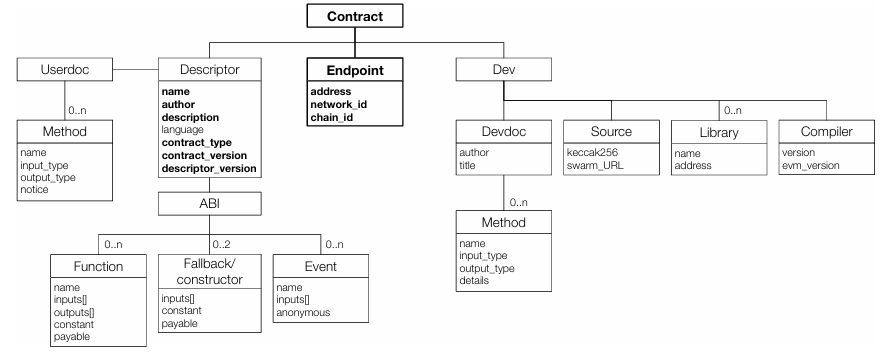
\includegraphics[width=1\textwidth]{resources/chapter-2/sc-model.png}
	\caption{Model deskripsi kontrak \parencite{guida2019supporting}}
	\label{image:sc-model}
\end{figure}

\begin{figure}[ht]
	\centering
	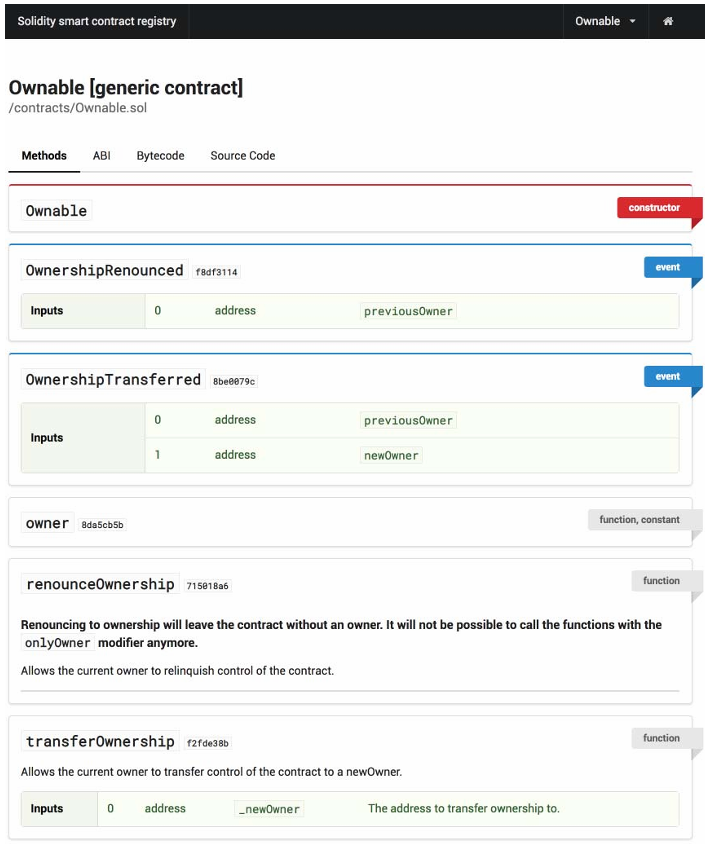
\includegraphics[width=0.7\textwidth]{resources/chapter-2/sc-registry.png}
	\caption{Tampilan Smart Contracts Registry \parencite{guida2019supporting}}
	\label{image:sc-registry}
\end{figure}

\begin{figure}[ht]
	\centering
	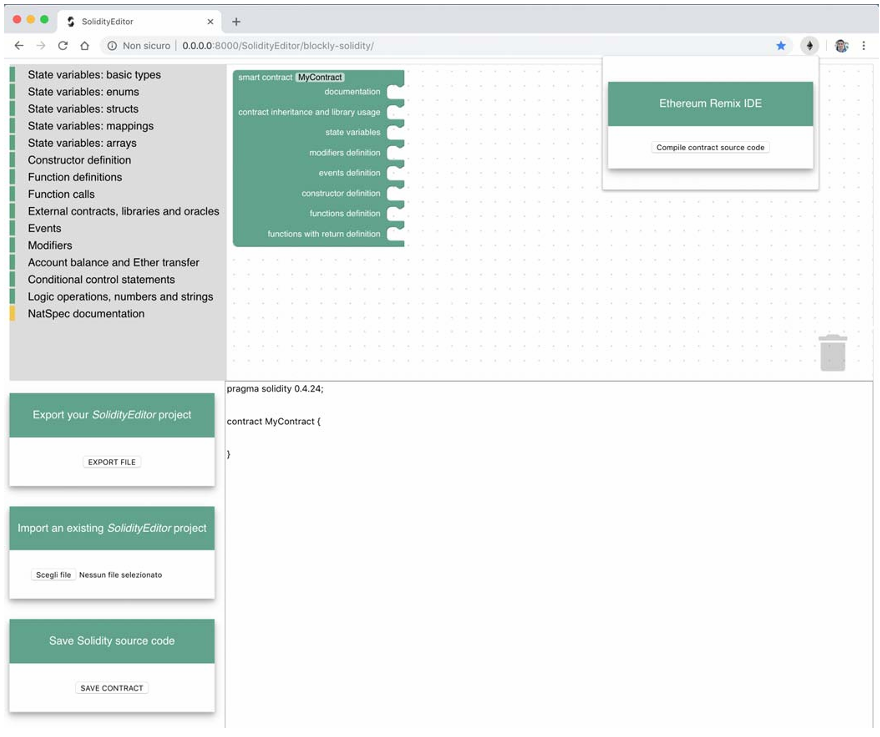
\includegraphics[width=0.7\textwidth]{resources/chapter-2/sc-editor.png}
	\caption{Tampilan Smart Contracts Visual Editor \parencite{guida2019supporting}}
	\label{image:sc-editor}
\end{figure}

\begin{figure}[ht]
	\centering
	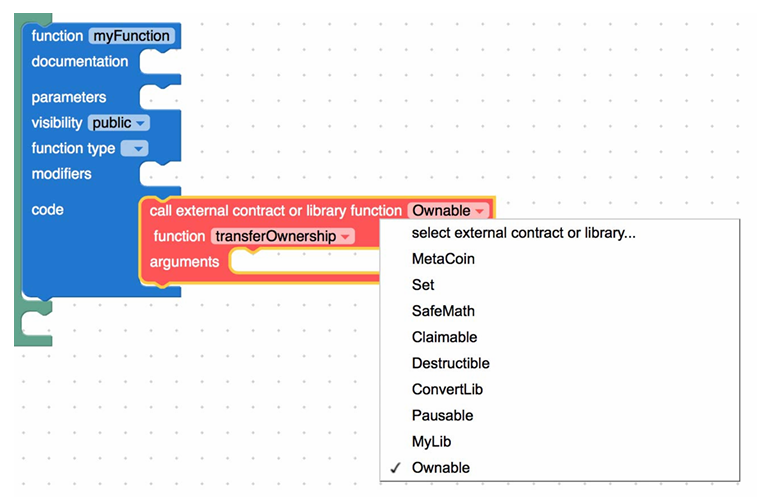
\includegraphics[width=0.7\textwidth]{resources/chapter-2/sc-editor-edit.png}
	\caption{Tampilan Smart Contract Selector \parencite{guida2019supporting}}
	\label{image:sc-editor-edit}
\end{figure}

\break

Penelitian ini menyoroti pentingnya deskripsi Smart Contracts yang memungkinkan pengembang untuk mencari dan menggunakan kontrak yang ada tanpa harus membaca kode sumbernya secara langsung. Model deskripsi kontrak yang diusulkan pada gambar \ref{image:sc-model} mencakup metadata yang sudah ada, seperti ABI dan dokumentasi, serta informasi teknis tambahan untuk memfasilitasi pencarian dan integrasi Smart Contracts. Selain itu, penelitian ini mengembangkan \textit{registry} Smart Contracts seperti yang ditunjukkan pada gambar \ref{image:sc-registry} dan \textit{editor} visual berbasis blok seperti yang ditunjukkan pada gambar \ref{image:sc-editor} dan gambar \ref{image:sc-editor-edit} untuk memudahkan pengembangan Smart Contracts yang lebih besar dan kompleks dengan cara yang lebih efisien dan dapat mengurangi kesalahan pemrograman.

\break

Implementasi ini menunjukkan bahwa penggunaan pendekatan berbasis visual, seperti \textit{editor} SolidityEditor, dapat mengurangi risiko kesalahan sintaksis, mempercepat pengembangan, dan memudahkan penggunaan kembali kode dengan mengintegrasikan pustaka kontrak eksternal seperti yang digunakan dalam studi kasus SmartTrainInsurance.
